Before starting with the measurements, we need to choose the optimal number of threads per thread block. The goal is to maximize SM thread occupancy.
The GPU used for CUDA acceleration is an RTX 3060Ti, whose compute capability is 8.6. From the computing capability, the following constraints are determined:
\begin{itemize}
  \item Maximum number of threads per SM: 1536
  \item Maximum number of blocks per SM: 16
  \item Maximum number of threads per block: 1024
  \item Maximum number of registers per block: 65536
  \item Maximum number of registers per thread: 255
  \item Maximum number of registers per SM: 65536
\end{itemize}
Furthermore, by compiling the kernel with \texttt{--ptxas-options=-v} argument, we determined that it needs 10 registers to be executed. We consider different number of block sizes:
\begin{itemize}
  \item $Block size = 32 threads$ \\ $\Rightarrow Number \; of \; blocks \; per \; SM \; = \; 1536 \; / \; 32 \; = \; 48$ \\ $\Rightarrow 48\;blocks\; > \; 16\;blocks/SM \Leftrightarrow SM \; can't \; be \; fully \; occupied$ \\ The actual number of threads per SM is $16\;blocks\;*\;32\;thread/block\;=\;512\;threads$ \\The occupancy level is $33\%$
  \item $Block size = 64 threads$ \\ $\Rightarrow Number \; of \; blocks \; per \; SM \; = \; 1536 \; / \; 64 \; = \; 24$ \\ $\Rightarrow 24\;blocks\; > \; 16\;blocks/SM \Leftrightarrow SM \; can't \; be \; fully \; occupied$ \\ The actual number of threads per SM is $16\;blocks\;*\;64\;thread/block\;=\;1024\;threads$ \\The occupancy level is $66\%$
  \item $Block size = 128 threads$ \\ $\Rightarrow Number \; of \; blocks \; per \; SM \; = \; 1536 \; / \; 128 \; = \; 12$ \\ $\Rightarrow 12\;blocks\; <= \; 16\;blocks/SM \Leftrightarrow SM \; can \; be \; fully \; occupied$ \\ The actual number of threads per SM is $12\;blocks\;*\;128\;thread/block\;=\;1536\;threads$ \\The occupancy level is $100\%$
  \item $Block size = 256 threads$ \\ $\Rightarrow Number \; of \; blocks \; per \; SM \; = \; 1536 \; / \; 256 \; = \; 6$ \\ $\Rightarrow 6\;blocks\; <= \; 16\;blocks/SM \Leftrightarrow SM \; can \; be \; fully \; occupied$ \\ The actual number of threads per SM is $6\;blocks\;*\;256\;thread/block\;=\;1536\;threads$ \\The occupancy level is $100\%$
  \item $Block size = 512 threads$ \\ $\Rightarrow Number \; of \; blocks \; per \; SM \; = \; 1536 \; / \; 512 \; = \; 3$ \\ $\Rightarrow 3\;blocks\; <= \; 16\;blocks/SM \Leftrightarrow SM \; can \; be \; fully \; occupied$ \\ The actual number of threads per SM is $3\;blocks\;*\;512\;thread/block\;=\;1536\;threads$ \\The occupancy level is $100\%$
  \item $Block size = 1024 threads$ \\ $\Rightarrow Number \; of \; blocks \; per \; SM \; =   \; \lfloor 1536 \; / \; 1024 \rfloor \; = \; 1$ \\ $\Rightarrow 1\;blocks\; <= \; 16\;blocks/SM \Leftrightarrow SM \; can \; be \; fully \; occupied$ \\ The actual number of threads per SM is $1\;blocks\;*\;1024\;thread/block\;=\;1024\;threads$ \\The occupancy level is $66\%$
\end{itemize}
In order to get maximum SM occupancy we choose a block size of $512$ threads, which guarantees the execution of $1536$ threads per SM. This needs a total of $1536*10=15360$ registers to be executed which is compatible with the constraints set by the computing capability of our GPU.

\begin{figure}
  \begin{center}
    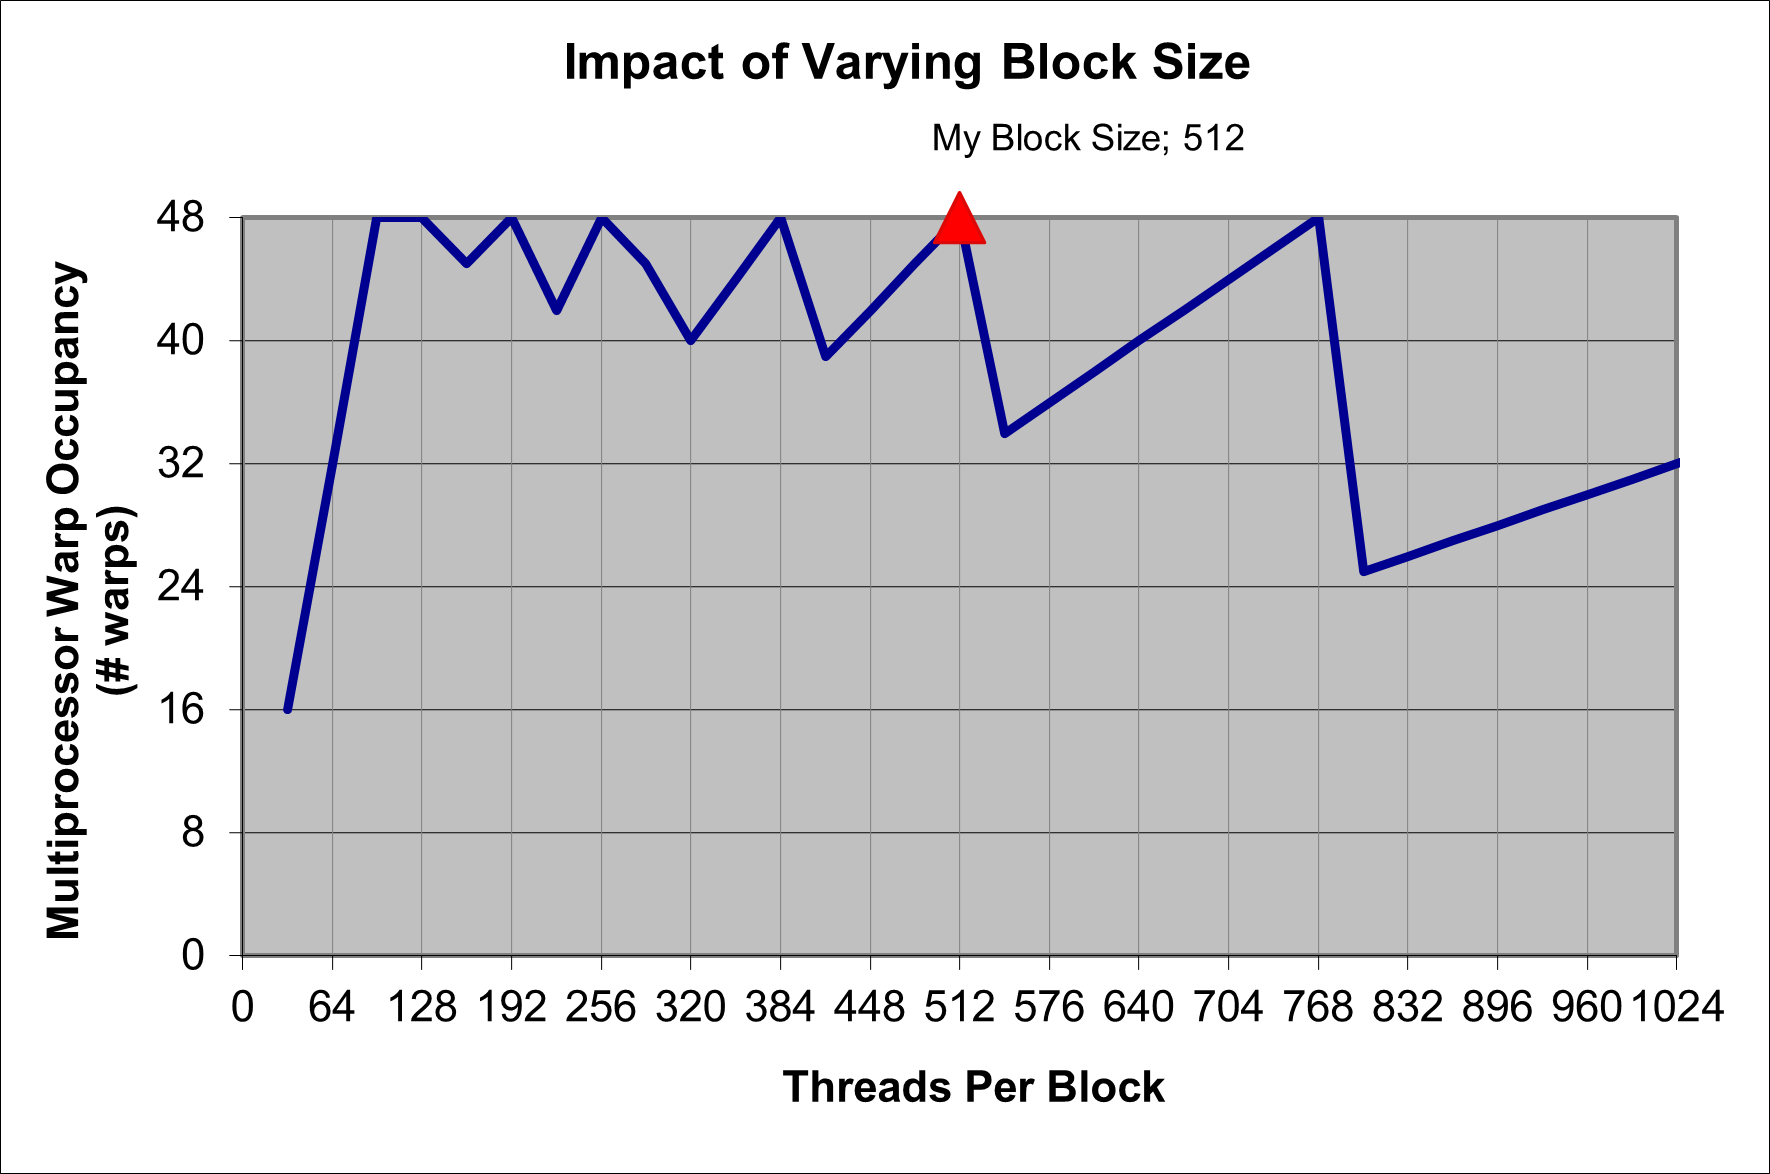
\includegraphics[scale=1]{img/Immagine1.png}
  \end{center}
  
  \caption{Variation of warp occupancy with respect to block size}
  \label{img:warp-occupacy}
\end{figure}